The calibration using cosmic ray muons was sufficient for initial data-taking with the electron beam, but the overall energy calibration of the ECal is optimal at higher energies. The ECal detects electrons from elastic scattering at the target that peak, after correction for shower leakage effects, at the beam energy. As the target is off centerline beam right, there are geometric effects that prevent elastically-scattered beam energy electrons from full coverage of the ECal.~\cite{szumila-vance_hps_2016} From simulation, the first column of crystals on beam right, and the five columns of crystals on beam left cannot be calibrated using elastically-scattered electrons. \\
\indent To calibrate the ECal using elastically-scattered electrons, we selected events where the seed hit crystal carried at least 60$\%$ of the overall cluster energy. The seed hit was also required to have carried greater than 450~MeV in the 2015 data (1.1~GeV for the 2016 dataset), to have triggered a Singles-1  event readout from the DAQ, and to have occurred in the optimal trigger timing window. The cluster energy was associated with the seed hit module for the calibration. The calibration uses an iterative procedure, by which the reconstructed peak energy is matched to that found by simulation (prior to energy corrections). For each peak, an iteration coefficient is found that reflects the ratio of the peak position measured in Monte Carlo to the peak position found for a particular iteration in the data. This ratio can be seen in Equation~\eqref{eq:feeiter}.

\begin{equation}
	\label{eq:feeiter}
	C_i = \dfrac{MC_{peak}}{data_{peak}}
\end{equation}

After each iteration, this ratio $C_i$ is applied to the to the original gain coefficient as well as any coefficient found from previous iteration. The data is re-processed applying these changes to the gains and clustering is re-run. This procedure continues until the correction coefficients found in a particular iteration are all less than 1$\%$. Crystals on the edge of acceptance with poorly resolved peaks were given an iteration coefficient of 1. After completion of the calibration (approximately 2-3 iterations)~\cite{szumila-vance_hps_2016}, the shower loss correction functions were applied to the reconstructed cluster energies. The final peak position for elastically-scattered electron clusters in the fiducial region of the ECal is shown in Figure

\begin{figure}[H]
  \centering
      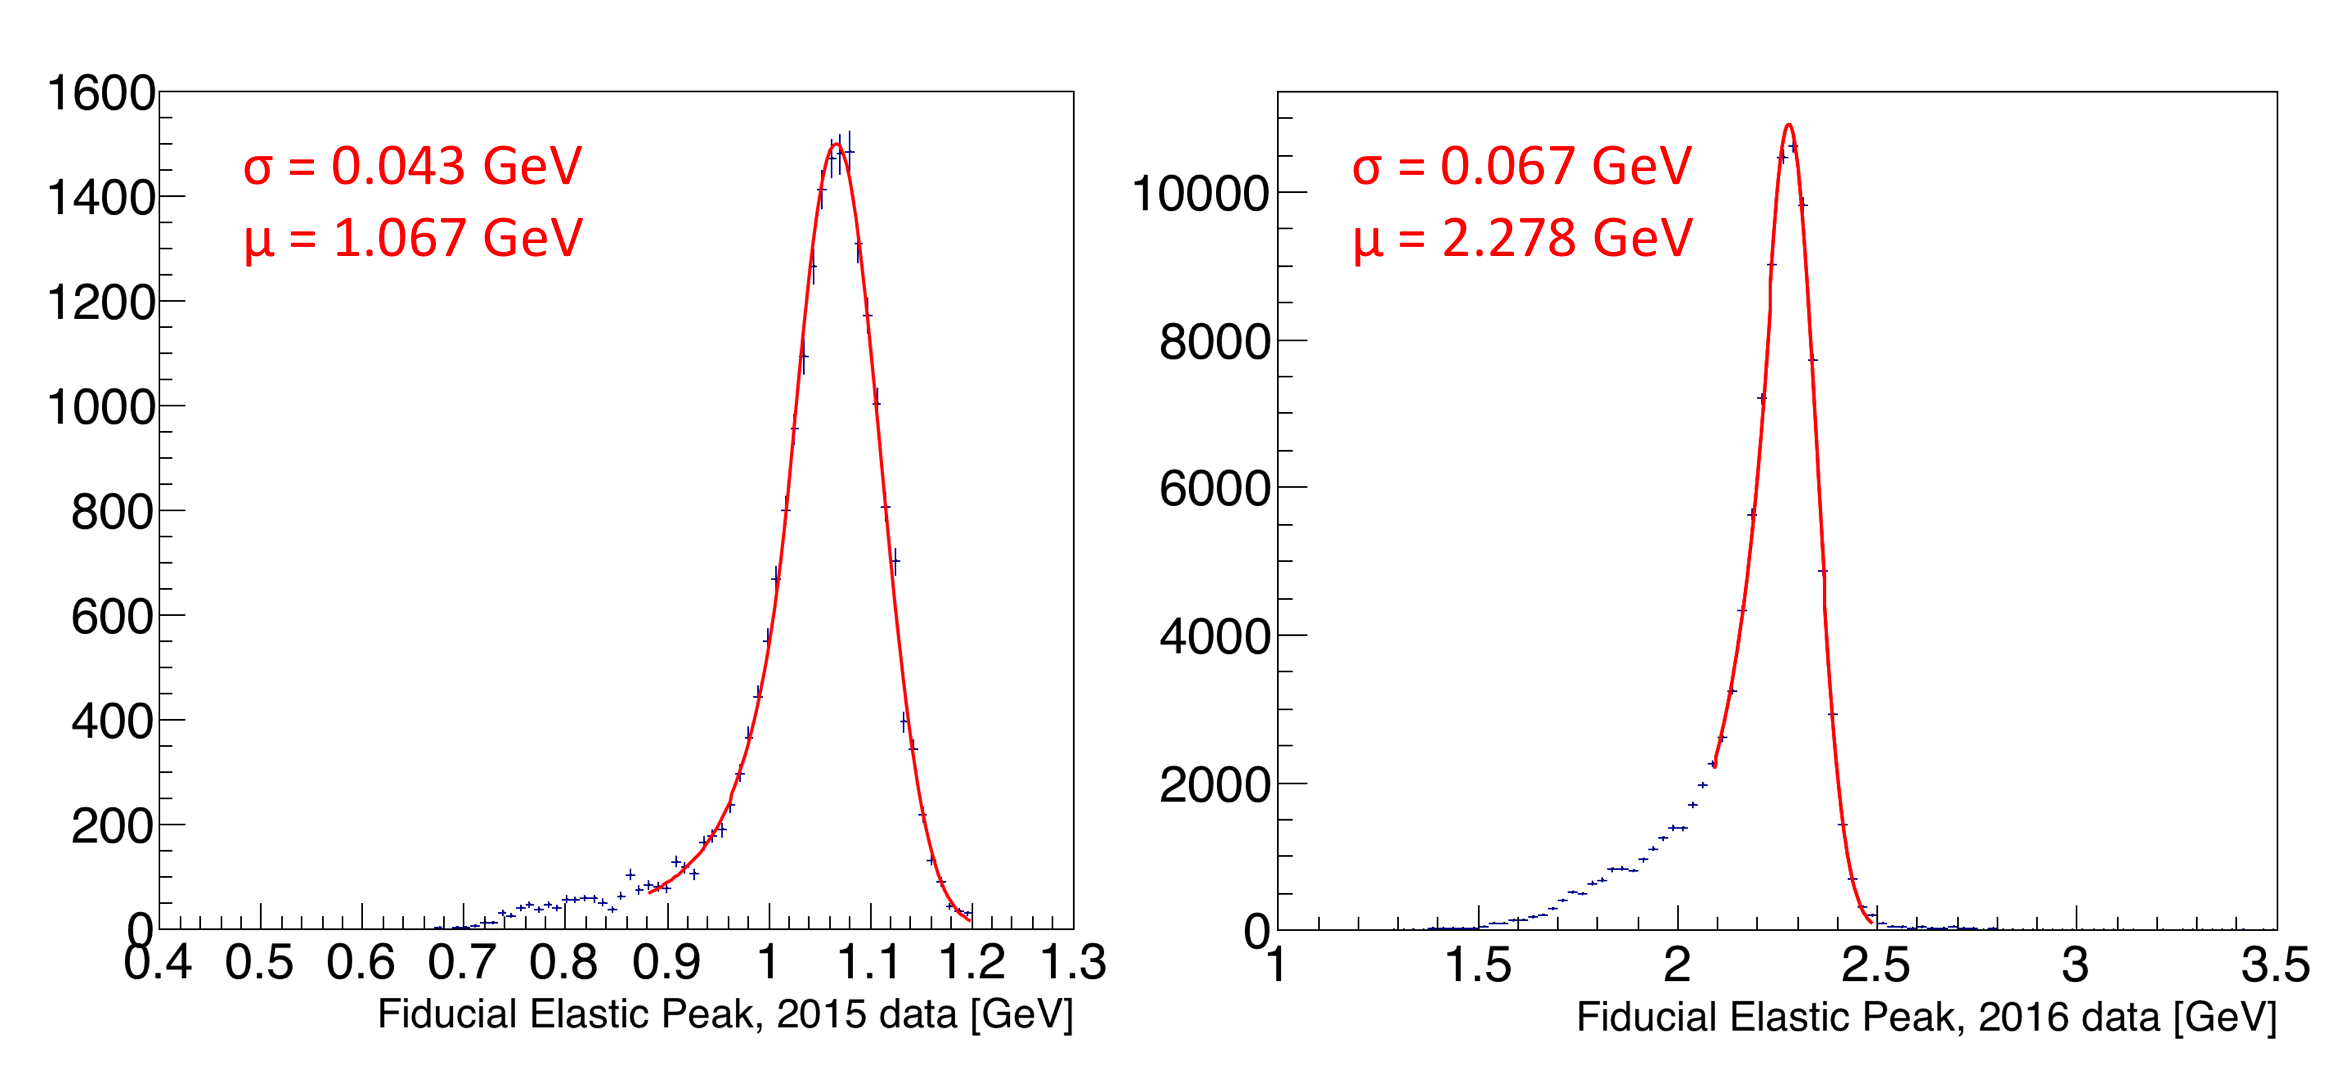
\includegraphics[width=0.9\textwidth]{pics/performance/feePeakFid.png}
  \caption[Reconstructed elastic peak in the ECal for the Engineering and Physics Runs]{Shown are the resultant fiducial peaks for the Engineering and Physics Runs on the left and right, respectively. The peaks are fit with a Crystal Ball function and the peak position and widths are indicated. }
  \label{Figure:FeeFidPeak}
\end{figure}

The energy resolution improves with the beam energy. The cluster energy spectrum is fit with a Crystal Ball function which contains a Gaussian component and a power law low energy tail. The ECal has an energy resolution of approximately 4$\%$ in the fiducial region at approximately 1~GeV and 2.9$\%$ at 2.3~GeV. \\
\indent The final gains obtained after calibration with elastically-scattered electrons were compared to the gains obtained with cosmics alone in order to check for systematic offsets. While no systematic offsets were found, the comparison between the low and high energy calibrations tells us that the initial energies used for the cosmic calibration are roughly accurate, but it is limited in telling us anything about the linearity of the gain between these two energies.~\cite{szumila-vance_hps_2016} If there was found to be any systematic offsets, these should be applied to the gains of the crystals that could not be calibrated using the elastically-scattered electrons due to acceptance, and the effects on the triggered data would need to be quantified. 

%\begin{figure}[H]
 % \centering
    %  \includegraphics[width=0.9\textwidth]{pics/performance/cosmicComp.png}
 % \caption[Gain comparison between cosmic and elastic calibration]{A comparison between the gains from he cosmic and elastic calibration is shown. Any overall systematic shift would need to be applied to crystals outside of the elastic calibration acceptance. }
%  \label{Figure:cosmicComp}
%\end{figure}
